\section{Audiocodierung}
\begin{center}
    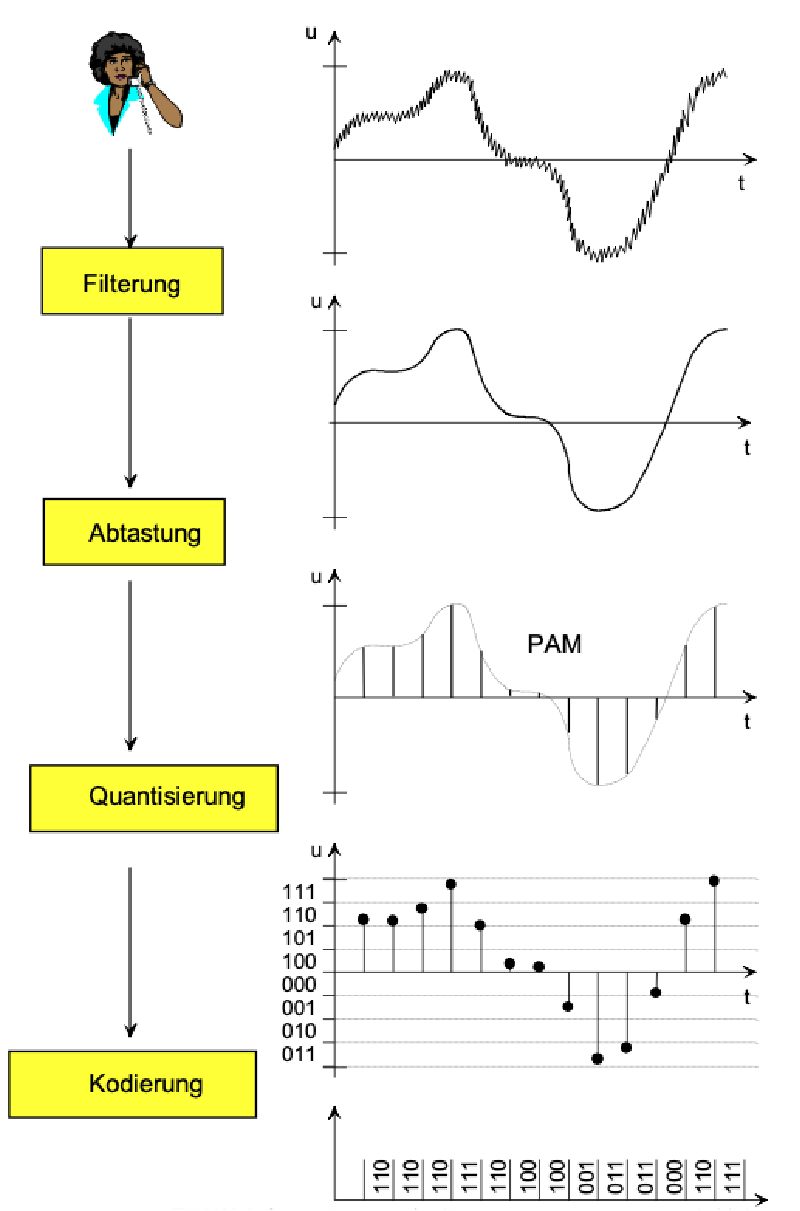
\includegraphics[scale=0.3]{a1}
\end{center}
\subsection{Filterung}
Mit Hilfe eines Filters werden die zu hohen und die zu tiefen
Frequenzen entfernt. Das Signal wird also auf einen hörbaren
Frequenzbereich (typischerweise 20-20kHz) begrenzt.
\subsection{Abtastung}
Abtastfrequenz muss mindestens doppelt so gross sein, wie die
höchste im analogen Signal vorkommende Frequenz (siehe
Abtasttheorem)
\begin{center}
    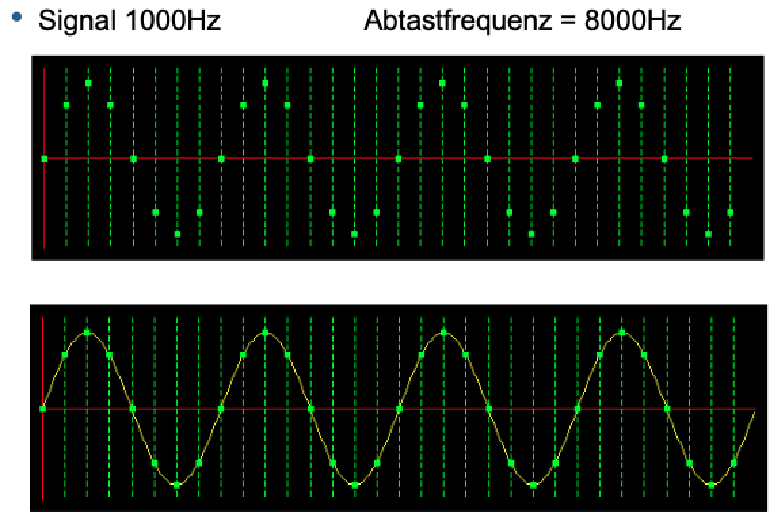
\includegraphics[scale=0.35]{a2}
\end{center}
\subsection{Quantisierung}
Anzahl Bit, die für die Quantisierung verwendet werden, bestimmt
die Anzahl Stufen, welche für die Messung der Amplitude zur
Verfügung stehen.
\\
\\
Die gemessenen Werte werden der nächsten Stufe zugeordnet
(gerundet). Dabei entsteht ein sogenannter \textbf{Quantisierungsfehler}.
\begin{center}
    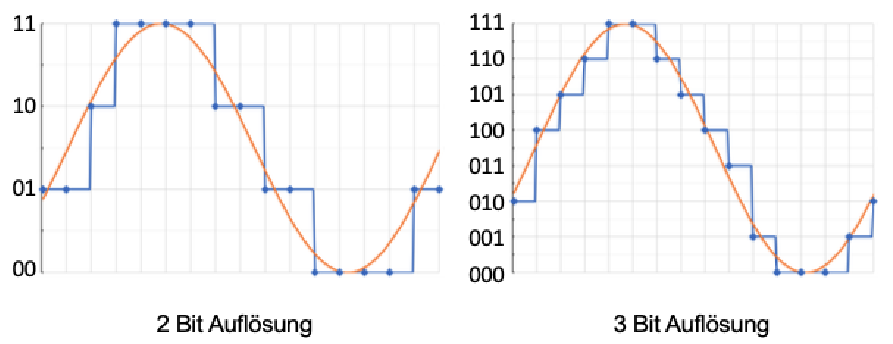
\includegraphics[scale=0.35]{a3}
\end{center}
Quantisierungsrauschen: Differenz Quantisierung und dem Signal
\\
\\
\\
Das \textbf{Quantisierungsrauschen} wird kleiner bei grösserer Anzahl
verwendeter Bits.
\begin{center}
    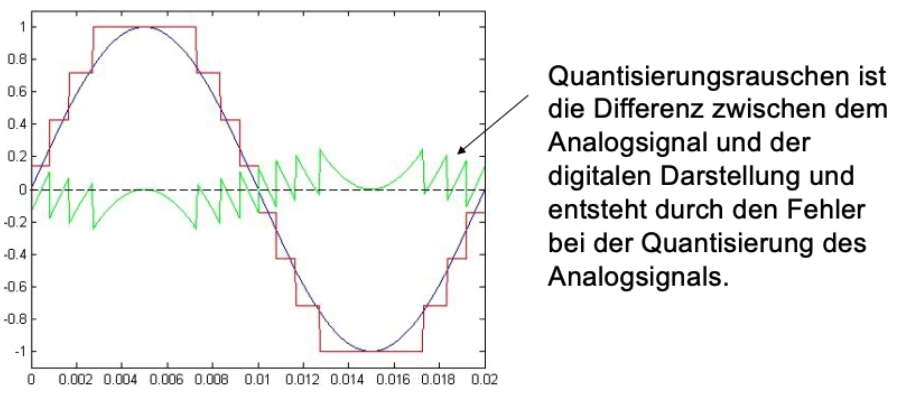
\includegraphics[scale=0.35]{a4}
\end{center}
\begin{itemize}
    \item \textbf{Mit jedem Bitanstieg} nimmt das Quantisierungsrauschen um \textbf{6dB} ab.
    \item Jede Bit-Zunahme bedeutet eine \textbf{Verdoppelung} der Anzahl Stufen und damit eine Halbierung des Quantisierungsrauschens.
\end{itemize}
\subsection{Codierung}
Jedem quantisierten Messwert wird ein Wert von einer bestimmten
Bitlänge zugeordnet. Typischerweise werden 16Bit zur Aufzeichnung von Audio in hoher
Qualität verwendet. (Professionell: 24Bit)
\\
\\
Aufgrund der Abtastrate entsteht somit ein Bitstrom, der berechnet
werden kann:

\begin{align*}
\text{Anzahl Bit pro Messwert (Sample)} \times \text{Abtastfrequenz} \\
\end{align*}

\subsubsection{PCM (linear Quantisiert)}
Bei jedem Stützwert wird ein absoluter Wert codiert und bei jedem Wert, wird die volle 
Anzahl Bits gebraucht.
\begin{center}
    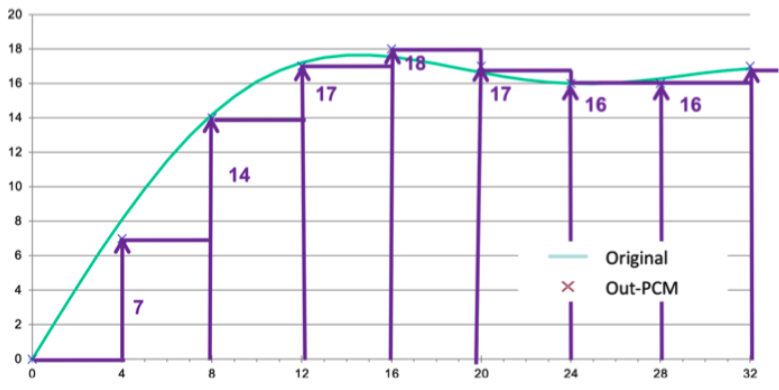
\includegraphics[scale=0.35]{a5}
\end{center}
\subsubsection{DPCM (Differential-PCM)}
Bei jedem Stützwert wird die Differenz zum vorherigen codiert.
\begin{center}
    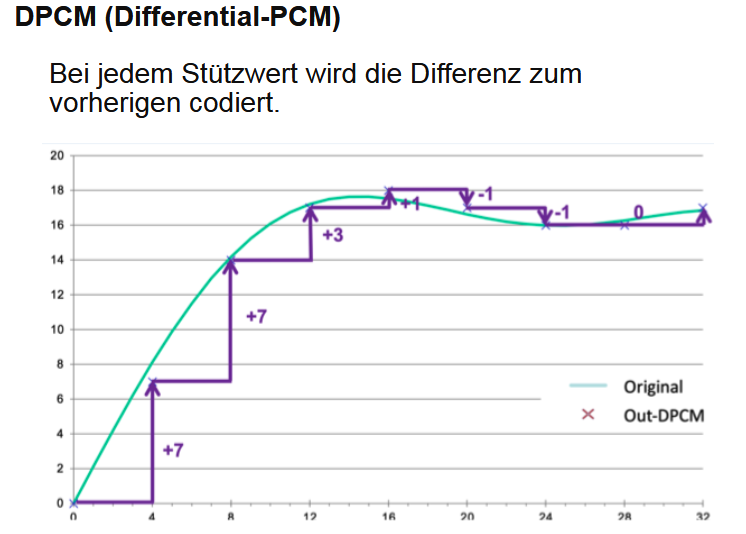
\includegraphics[scale=0.35]{a6}
\end{center}
\subsubsection{ADPCM (Adaptive-Differential-PCM)}
Nur Korrekturwert K wird codiert (Korrektur des vorherigen Korrekturwertes).
\begin{center}
    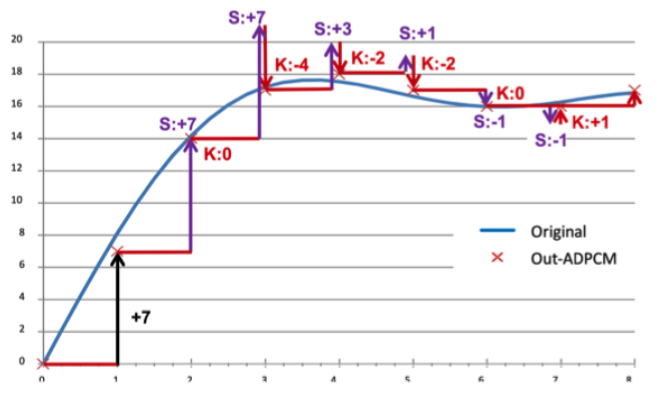
\includegraphics[scale=0.35]{a7}
\end{center}

\subsection{Abtastheorem}
Die Abtastfrequenz muss mindestens doppelt so gross sein, wie die höchste im analogen Signal 
vorkommenden Frequenz.
\begin{align*}
    f_{\text{abtast}} > 2 \times f_{\text{max}}
\end{align*}

\subsection{Beispiel}
\begin{center}
    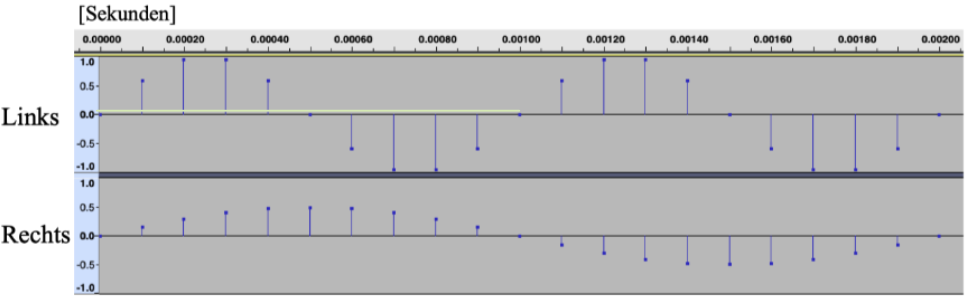
\includegraphics[scale=0.35]{a8}
\end{center}
\subsubsection{Abtastfrequenz finden}
Samples (blaue Punkte) für eine Periode $T$ zählen (hier 10).
\begin{align*}
    f = 1 / T = 1 / 0.01s = 100Hz
\end{align*}
\begin{align*}
    f_{\text{abtast}} = (1 / T) \times \text{n-samples} = 1000Hz \times 10 = 10000Hz
\end{align*}
\subsubsection{dB Unterschied}
Halbierung der Lautstärke/Amplitude entspricht einer Reduktion von 6dB. 
\subsubsection{Filesize}
16-Bit-Tiefe = 2 Byte/Sample
\begin{align*}
    \text{Filesize} = (\text{Abtastfrequenz} \times \text{Länge} + 1) \times \text{Byte/Sample} \times \text{Anzahl Kanäle} + \text{Header}
\end{align*}
Sollte ca. das gleiche sein wie:
\begin{align*}
    \text{Filesize} = \frac{\text{Abtastfrequenz} \times \text{Länge} \times \text{Auflösung} \times \text{Anzahl Kanäle} + \text{Header}}{8}
\end{align*}